\documentclass[twocolumn, a4paper]{UECIEresume}

\usepackage[dvipdfmx]{graphicx}
\usepackage{graphicx}
\usepackage{amsmath}
\usepackage{txfonts}
\usepackage{url}
\usepackage{enumerate}

\setlength\intextsep{0pt}
\setlength\textfloatsep{0pt}


\title{複数人で使用可能な3Dアイデアノートシステムの提案と実装}
\date{平成 29 年 9 月 26 日}
\affiliation{情報学専攻 メディア情報学プログラム}
\supervisor{田野 俊一 教授,橋山 智訓 准教授}
\studentid{1630012}
\author{猪膝 孝之}
%\headtitle{平成 yy 年度 総合情報学科 卒業論文中間発表}
%\headtitle{平成 yy 年度 総合情報学科 卒業論文発表}
\headtitle{平成 29 年度 情報学専攻 修士論文中間発表}
%\headtitle{平成 yy 年度 総合情報学科 修士論文発表}



\begin{document}
\maketitle

\section{はじめに}
アイデアはふとしたときに思い浮かぶことがあり、私達はそれを紙に書き留めたり、PCを利用してメモを取ることがある。しかし、アイデアが思い浮かぶのは座って作業しているときだけではなく、外で歩いているときや、机やホワイトボード等がないような場面でも突然思い浮かぶことがある。また、友人と話し合いをしているときにアイデアが連鎖的に生まれることがある。

近年、HMD(Head Mounted Display)が普及してきた。現在、HMDに関する多くの研究は一人で特定の場所において使うことが想定されている。現状では外などの広い空間を利用し、複数人で利用することを想定した研究やアプリケーションは少ない。本研究は実世界の広い空間上の任意の場所にメモを残すことができ、複数人で利用できるようなシステムの提案と実装を行う。

\section{関連研究}
椎尾ら\cite{tex1,tex2}は仮想の手書きメモによるコミュニケーションをウェアラブルコンピュータにより実現する空気ペンを試作した。問題点としては、同時に複数人で使用できないことや、使用できる範囲がRFIDタグがついた床上のみなので場所が限定されることが挙げられる。

また、高山ら\cite{tex3,tex4}は実世界のどのような時間・場所であっても、ユーザが思い浮かんだふとしたアイデアを、生起を誘発したコンテキストに対応づけて保存し、それを他のユーザと共有できるシステムを作成した。問題点としては、多くの機器を装着しなければならないので持ち運びが大変であることや、操作が複雑なので慣れるのに時間がかかることが挙げられる。

長田ら\cite{tex5}はスマートグラスを用いた仮想空間への手書き情報共有システムを提案した。問題点としては、指のみの操作だとできることが限定されることが挙げられる。


\section{本研究のコンセプト}
先行研究では一人で使用をすることを想定していたり、使用できる場所が限定される、持ち運びが難しい、操作が複雑等の問題点があった。そこで、本研究は以下のようなシステムを提案する。
\begin{enumerate}[(1)]
 \item 複数人で話し合ってアイデアを生み出し、お互いのメモを共有することができる。
 \item 実世界の広い空間上の任意の場所にメモを置くことができ、どこでも場所を選ばず利用できる。
 \item 簡単な操作で直感的に様々な入力ができる。
\end{enumerate}

\section{提案するシステム}
ハードウェアは可搬性を考慮して、マイクロソフト社のHoloLens\cite{tex6}を使用する。

\subsection{全体設計}
本研究のコンセプトで述べた(1)、(2)、(3)を踏まえると、システムとして必要な機能は大きく分けて、メモを入力、メモを操作、メモを共有の三つである。以下にそれぞれについて詳細を述べる。

\subsection{メモを入力}
実世界の任意の3D空間上に図形や文字のメモを残す。また、これらに加えて音声によるメモも残すことも実現する。3D空間上に文字によるメモをそのまま残す場合、見る方向によっては文字として見えないと問題が発生することが考えられる。これを解決するために3D空間上に仮想平面を用意してその平面上に文字を描き、表示をする際に回転させて相手の方に面を向けるという手法を提案する(図\ref{fig:memokaiten})。また、文字を描き、この情報を点として3D空間上に残すという手法を提案する。見る際は3D空間上に残した点のメモをタップすることで文字を表示する。この手法により、どの方向から見ても文字として見ることを可能にする。

\begin{figure}[h]
  \begin{center}
    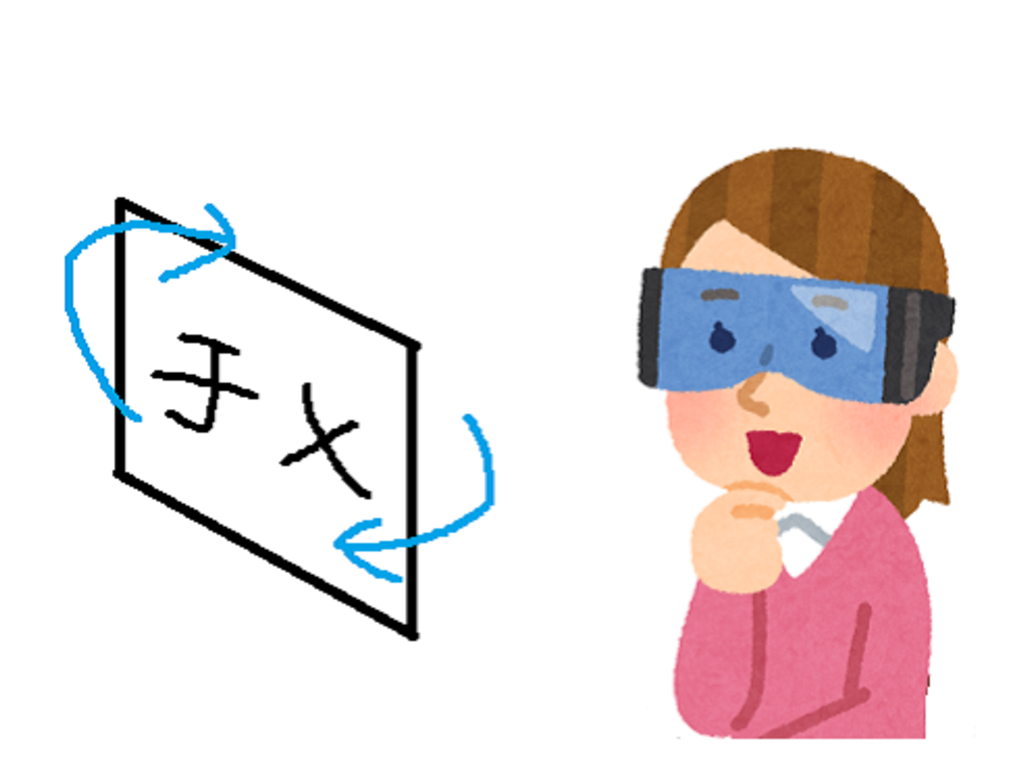
\includegraphics[clip,height=4.0cm,width=6.0cm]{./memokaiten.eps}
    \caption{仮想平面上に描き回転}
    \label{fig:memokaiten}
  \end{center}
\end{figure}


\subsection{メモを操作}
広い空間上にメモを残す場合、遠くに配置してあるメモをどうやって選択、移動、削除するかという問題が発生する。そこで、手元に部屋全体を縮小したものを用意して、メモを操作する手法を提案する(図\ref{fig:roomshukusho})。

\begin{figure}[h]
  \begin{center}
    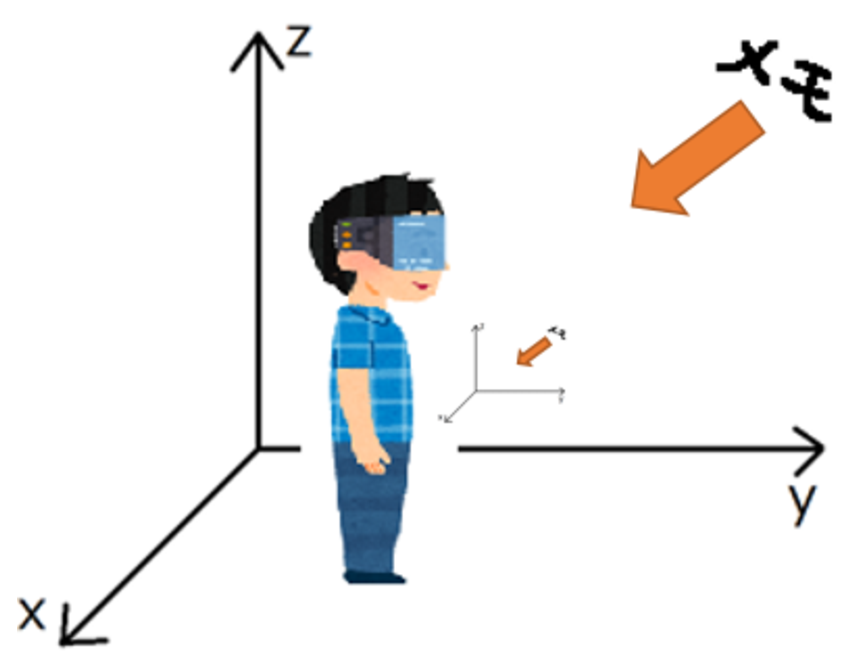
\includegraphics[clip,height=4.0cm,width=5.0cm]{./roomshukusho.eps}
    \caption{部屋全体を縮小して、手元でメモを操作}
    \label{fig:roomshukusho}
  \end{center}
\end{figure}

\subsection{メモを共有}
実世界の任意の3D空間上に残したメモを他人に見せるには、HoloToolkit\cite{tex7}のSharing\cite{tex8}という機能を利用し、Sharing用のサーバを介して空間の共有を行う。HoloToolkitとはHoloLens向けのアプリを効率的に開発するための機能を含んだツールキットのことである。また、対面にいる人だけでなく、遠隔にいる人にもメモを共有できるようにする。

\section{システムの試作}
本システムを作成する前に、実際に動作するかどうか確認を行うために3D描画システムの試作を行った。

\subsection{実装環境}
ハードウェアはHoloLensを利用し、開発環境はWindows10でUnity\cite{tex9}を使用した。また、Unity用のHoloLens向けのツールキットであるHoloToolkit-Unityの導入を行った。

\subsection{動作確認}
3D描画システムの試作を行い、HoloLens上でシステムを動かして、動作を確認した。3D空間上でタップアンドホールドをすると描画が開始され、ホールドを解除すると描画を終了するようにした。3D空間上で手前から奥に線を引くことができることも確認できた。線が表示される位置がタップアンドホールドした位置より少し離れた場所に表示されているので、今後調整する必要があると考えられる。また、図\ref{fig:rittai}のように3D空間上に配置した仮想平面上に文字を描いて、自分の方向に面を向けて表示できることも確認できた。

\vspace{0.5zh}

\begin{figure}[h]
  \begin{center}
    \includegraphics[clip,height=4.0cm,width=7.0cm]{./tegakimoji.eps}
    \caption{仮想平面上に描いた文字を自分に向けて表示}
    \label{fig:rittai}
  \end{center}
\end{figure}

\vspace{-1zh}
\vspace{-1zh}

\section{まとめ}
3D空間上の任意の場所にメモを置くことができ、複数人で使用できる3Dアイデアノートシステムの提案を行った。

今後はメモの共有に関する予備実験、本システムの実装、本実験、評価を行っていく予定である。

\vspace{-1zh}

{\small
\begin{thebibliography}{99}
\bibitem{tex1}
        山本, 椎尾:
        空気ペン―空間への描画による情報共有-;
        情報処理学会全国大会講演論文集,
        {\bf Vol.59}, No.4, pp.39-40(1999).
\bibitem{tex2}
	椎尾, 山本:
	コミュニケーションツールのための簡易型ARシステム;
	コンピュータソフトウェア, 
        {\bf Vol.19}, No.4, pp.246-253(2002).
\bibitem{tex3}
	高山, 瑞慶山, 田野, 岩田, 橋山:
	実世界コンテキスト・情報を用いたユビキタスインフォーマルコミュニケーションの実装と評価;
	ヒューマンインタフェースシンポジウム2005,
        pp.955-958(2005).
\bibitem{tex4}
        Tano, S., Takayama, T., Iwata, M. and Hashiyama, T.:
        Wearable Computer for Ubiquitous Informal Communication;
        Sixth International Workshop on Smart Appliances and Wearable Computing-IWSAWC 2006-(at 26th IEEE International Conference on Distributed Computing Systems ICDCS),
        pp.1-8(2006).
\bibitem{tex5}
        長田, 佐々木, 島田, 佐藤:
        スマートグラスを用いた仮想空間への手書き情報共有システム;
        情報処理学会第77回全国大会論文集,
        3-205, 206(2015).
\bibitem{tex6}
        Microsoft Inc:
        HoloLens;
        \textless\url{https://www.microsoft.com/ja-jp/hololens}\textgreater2017年9月21日アクセス.
\bibitem{tex7}
        Microsoft Inc:
        HoloToolkit;
        \textless\url{https://github.com/Microsoft/HoloToolkit-Unity}\textgreater2017年9月21日アクセス.
\bibitem{tex8}
        HoloToolkit-UnityのSharingの仕組みをできるだけ簡単に理解する; 
        \textless\url{http://qiita.com/miyaura/items/da1d7bd253c3299327ba}\textgreater2017年9月21日アクセス.
\bibitem{tex9}
        Unity Technologies Inc:
        Unity;
        \textless\url{https://unity3d.com/jp/unity}\textgreater2017年9月21日アクセス.

\end{thebibliography}
}
\end{document}